% Online Resource 1 for "Temporal Profiles of Online Attention: Measuring
% Persistence, Recency, and Re-Emergence with TH-EE".
%
% Compiles standalone. Numbers are generated by
%   python analysis/wikipedia_collect.py --alts
%   python analysis/wikipedia_analysis.py
%   python analysis/sequence_baselines.py
%   python analysis/make_wikipedia_figures.py
% and are transcribed here from wikipedia_results.json and
% sequence_baseline_results.json.

\documentclass[11pt]{article}
\usepackage[margin=1in]{geometry}
\usepackage{amsmath,amssymb}
\usepackage{booktabs}
\usepackage{graphicx}
\usepackage{array}
\usepackage{xurl}
\usepackage[colorlinks=true,linkcolor=blue,citecolor=blue,urlcolor=blue]{hyperref}
\newcommand{\THGEE}{\operatorname{TH\mbox{-}GEE}}
\graphicspath{{../analysis/figures/}}
 
\title{Online Resource 1\\
\large An event-level replication of the TH-EE temporal profiles\\
using Wikipedia pageview series}
\date{}

\begin{document}
\maketitle

\section{Purpose}
\label{sec:or1_purpose}

The YouTube application in the main text anchors engagement to \emph{publication}
time. A quarterly value is therefore the eventual observed engagement of the
videos published in that quarter, not the audience activity that occurred during
it (main text, Sections 4.2 and 6.3). The main text states that direct
measurement of audience-level persistence or re-engagement would require
repeated engagement snapshots or event-level interaction records, and Section
5.4 defers the sequence-oriented baselines (Kleinberg burst scores, change-point
statistics, Hawkes intensities) on the same grounds.

This Online Resource supplies event-level records for the same 37 topics and
uses them to answer two questions the main text leaves open:

\begin{enumerate}
\item[\textbf{OR1.}] Do the temporal profiles computed from event-level audience
      activity agree with the publication-cohort profiles reported in the main
      text?
\item[\textbf{OR2.}] Does the Re-Emergence Index agree with sequence-oriented
      methods designed for event-level data, once such data are available?
\end{enumerate}

The replication is a construct check on the measurement framework. It is not a
new empirical claim about Wikipedia readers, and it does not alter the main
text's substantive conclusion that debunked-claim cohorts are temporally
heterogeneous.

\section{Data}
\label{sec:or1_data}

The Wikimedia REST pageviews API serves daily per-article view counts for
Wikipedia from 2015-07-01 onward. Counts are requested for the English
Wikipedia, all access methods (desktop, mobile web, mobile app), and the
\texttt{user} agent class, which excludes self-identified automated traffic;
2015-07-01 is both the first day the endpoint serves and the first day the agent
classification is available. The frozen horizon is 2015-07-01 to 2026-06-30
(4{,}018 days). No API key or quota is involved, and the collection script issues
one request per article-year.

Each of the 37 topic-search terms used in the main text is mapped to the English
Wikipedia article whose subject is that topic. Because Wikimedia records a
pageview against the \emph{requested} title, a redirect title carries its own
attention series; where a topic name redirects to an article on the same subject
under a different name the target is used, and where it redirects to a broader or
different subject the topic-named redirect is used instead, because its series is
specific to the topic. Each mapping is labelled with a fidelity grade:
\emph{high} when the article's subject is the topic, \emph{medium} when the
article contains the topic but is broader, and \emph{low} when the closest
available article is substantially broader than the search term. Results are
reported for all 37 topics and again restricted to the high-fidelity subset, so
that the effect of imperfect mapping is visible rather than assumed away.
Table~\ref{tab:or1_mapping} lists the mappings.

\section{Trace construction}
\label{sec:or1_traces}

Equation~1 of the main text is applied with a single interaction type. A pageview
is the interaction, $w_{\mathrm{pageview}} = 1$, and $t_{\tau}$ is the number of
days in window $\tau$, so

\begin{equation}
E_{\tau}(c) \;=\; \frac{\text{pageviews of article } c \text{ in window } \tau}
                       {\text{days in window } \tau}
\label{eq:or1_window}
\end{equation}

is the mean daily pageview rate. This is window-length independent and lands
every topic on the same grid. Windows are 90 days, the main text's primary
specification, anchored at 2015-07-01; the trailing partial window is dropped.
The recency coefficient $\gamma = 0.1$, the dormancy requirement $d = 2$, and the
per-topic activity threshold $q_h$ (the 25th percentile of a topic's nonzero
window scores) are carried over unchanged from the main text.

\subsection{Two indicators do not transfer unchanged}
\label{sec:or1_indicators}

Active-window coverage, the main text's scale-free persistence indicator, is
degenerate on pageview data. A YouTube window is zero when nobody published in
it; a Wikipedia window is essentially never zero, because a live article always
draws some traffic. Coverage is consequently at or near 100\% for nearly every
topic, and the $q_h$-based active fraction is approximately 75\% for every topic
by construction, since $q_h$ is defined as a within-topic quartile. Both are
reported below and both are uninformative on this data. This is a property of the
indicator meeting a denser data source, not a failure of the measurement.

The scale-free persistence quantity that does transfer is the ratio of the
Geometric Persistence Score to the arithmetic mean of the same trace,

\begin{equation}
\mathrm{G/A} \;=\; \frac{P_h(c)}{\frac{1}{T}\sum_{\tau=1}^{T} E_{\tau}(c)}
\;\in\; (0,1],
\label{eq:or1_ga}
\end{equation}

which equals 1 exactly when the trace is flat and falls toward 0 as engagement
concentrates into few windows. It is built only from quantities already in the
main text --- $P_h$ and the arithmetic-mean baseline of Section 4.5 --- it is
order-invariant like $P_h$, and it is invariant to rescaling the trace, so it is
comparable across platforms with very different engagement magnitudes. It also
reproduces the RQ1 separation directly: on the four construct traces of main-text
Table~3 it is $0.095$ for the acute burst against $0.996$ for the continuous
trace, the same order-of-magnitude separation $P_h$ itself produces there. All
cross-platform comparisons below use G/A, the recency ratio $\THGEE/P_h$, $R_h$,
and the reactivation count.

\subsection{Horizon matching}
\label{sec:or1_horizon}

Wikipedia series all begin on 2015-07-01, whereas each YouTube trace begins at
its own oldest sampled video, giving spans from 1.5 to 19.7 years. Comparing them
directly would confound the measures with the time axis. The primary comparison
therefore recomputes the YouTube publication-cohort traces on the \emph{same}
window grid restricted to 2015-07-01--2026-06-30, so both platforms have
identical $T$ and identical window boundaries. Profiles on the main text's own
full-span axis are reported alongside for reference.

Two consequences of the 2015-07 floor should be stated plainly. First, topics
whose activity peaked earlier --- notably the acute exemplars \emph{harlem shake}
(2013) and \emph{gangnam style} (2012) --- are observed only in their post-peak
tail on both platforms, so the replication cannot test the acute construct at its
peak. Second, per-article pageviews before 2015-07 are not available from any
Wikimedia API, so this floor cannot be lowered.

\section{Sequence-oriented baselines}
\label{sec:or1_baselines}

Daily pageviews are the event-level sequences that main-text Section 5.4
identifies as a prerequisite for burst and change-point methods, so both are run
here. Each is implemented directly from its source paper.

\paragraph{Kleinberg's burst automaton.}
The batched-stream formulation of Kleinberg's model is used: day $t$ contributes
$r_t$ views of the article out of $d_t$ views of the whole 37-article corpus, and
state $i$ has expected share $p_i = \min(p_0 s^i, 1-\epsilon)$ where
$p_0 = \sum_t r_t / \sum_t d_t$ is the article's baseline share. Using the corpus
as the denominator makes a burst a rise \emph{relative to the corpus}, which
absorbs Wikipedia-wide weekly and seasonal traffic cycles that would otherwise be
detected as bursts in every series simultaneously. The emission cost is the
negative binomial log-likelihood, moving up $j-i$ states costs
$(j-i)\gamma \ln n$, and bursts are the maximal runs of state $\geq 1$ in the
Viterbi path. Parameters are Kleinberg's defaults, $s = 2$ and $\gamma = 1$, with
three states (a base state and two burst levels).

\paragraph{PELT change-point detection.}
Exact change-in-mean segmentation with an $L_2$ cost on $\log(1+\text{views})$,
using the PELT pruning rule, with penalty
$\beta = 4\sigma^2 \ln n$ and $\sigma$ estimated from the median absolute
successive difference, which is robust to the jumps being detected. The minimum
segment length is 14 days, which keeps PELT to its intended role: a shift lasting
under two weeks is a burst, and is the other detector's business.

\paragraph{Verification.}
Both estimators, the G/A ratio, and the trace builder are checked against series
whose answers are known by construction in
\texttt{analysis/test\_sequence\_baselines.py}: Kleinberg recovers two injected
bursts to within three days and reports none in a stationary series or in a rise
proportional to the corpus; PELT locates an injected mean shift exactly and
reports none in a stationary or constant series; and the reduction identity
$\THGEE(\gamma{=}0) = P_h$ of main-text Equation~13 is re-exercised on this code
path.

\section{Results}
\label{sec:or1_results}

Table~\ref{tab:or1_mapping} gives the topic-to-article mapping and
Table~\ref{tab:or1_profiles} the event-level profiles under the primary
specification. Figure~\ref{fig:or1_exemplars} shows the quarterly traces of the
five featured topics of main-text Table~4.

\begin{figure}[htbp]
\centering
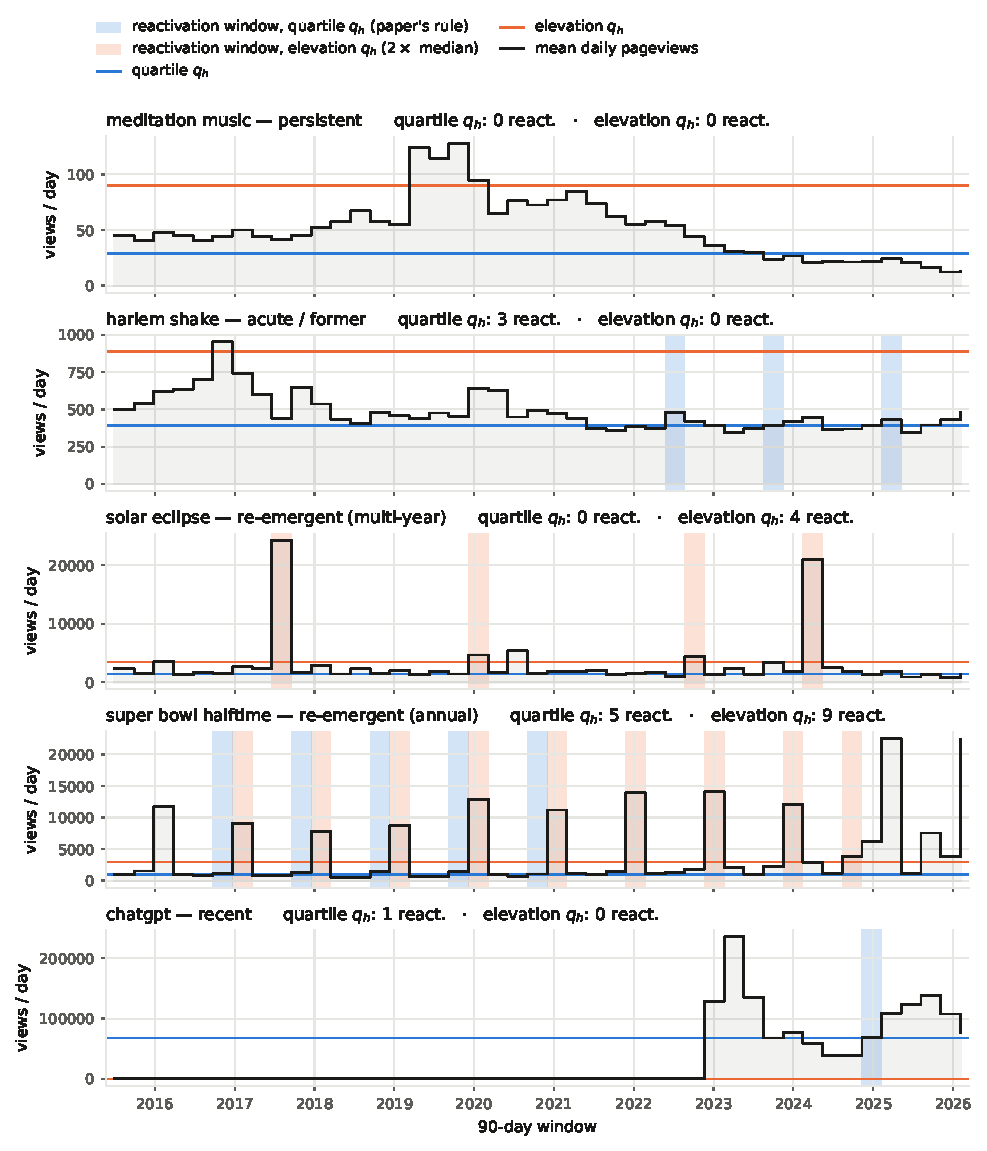
\includegraphics[width=\linewidth]{wikipedia_exemplars.pdf}
\caption{Event-level quarterly attention for the five featured topics, the
counterpart of main-text Figure~1. Shading marks qualifying reactivation
windows; the dotted line is $q_h$. The two eclipse spikes in the third panel are
the point discussed in Section~\ref{sec:or1_qh}: they are visually the clearest
returns in the dataset, and $R_h = 0$ for them.}
\label{fig:or1_exemplars}
\end{figure}

\subsection{OR1: agreement with the publication-cohort profiles}
\label{sec:or1_agreement}

Table~\ref{tab:or1_agreement} reports the rank agreement across seven
specifications; Figure~\ref{fig:or1_rankrank} shows the primary one topic by
topic. The result is that agreement is \emph{weak and specification-dependent},
and the three components behave differently.

\paragraph{Persistence.}
On the primary specification the correlation is $\rho = +0.43$ ($p = 0.008$;
$+0.50$ on high-fidelity mappings alone). This is the strongest single agreement
in the table, but it does not survive the own-span control: restricting each
trace to begin at its first active window drops it to $\rho = +0.19$
($p = 0.25$). The agreement is therefore carried substantially by the leading
zeros --- articles created inside the horizon, topic cohorts whose sampled videos
begin late --- rather than by the shape of the active portion of the trace. This
is the same zero-padding sensitivity that \texttt{robustness.py} documents for
the YouTube traces, now visible across platforms.

\paragraph{Recency.}
The recency ratio is the most consistently positive component, ranging from
$\rho = +0.28$ to $+0.43$ on six of the seven specifications and reaching
significance at 30-day ($+0.43$, $p = 0.008$) and 7-day ($+0.40$, $p = 0.015$)
windows. Where engagement mass sits within the horizon is thus partly a property
of the topic rather than of the platform.

\paragraph{Re-emergence.}
Re-emergence does not transfer. $R_h$ ranges from $\rho = +0.06$ to $+0.24$ and
the reactivation count from $-0.14$ to $+0.20$; neither reaches significance on
any specification.

\paragraph{A reliability ceiling makes the last result interpretable.}
Weak correlations could mean the measures disagree across platforms, or simply
that they are unstable. These are distinguished by asking how well the YouTube
profile agrees \emph{with itself} when computed on the two different time axes
used here (its own full span, and the matched 2015-07 horizon). It agrees at
$\rho = 0.47$ for persistence and $0.47$ for recency, but at $\rho = 0.89$ for
$R_h$ and $0.84$ for the reactivation count. So:

\begin{itemize}
\item For persistence and recency, the cross-platform agreement observed here
      ($0.43$ and up to $0.43$) is at essentially the same level as the YouTube
      measure's own stability under a change of time axis. These components
      transfer about as well as they replicate.
\item For re-emergence, the YouTube measure is highly stable internally
      ($0.84$--$0.89$) and yet uncorrelated with its event-level counterpart.
      This is a genuine disagreement, not noise.
\end{itemize}

The publication-cohort proxy is therefore weakest precisely where the main text
relies on it most heavily. Section~\ref{sec:or1_qh} shows that a substantial part
of this gap is attributable to the activity threshold rather than to the
construct.

\begin{figure*}[htbp]
\centering
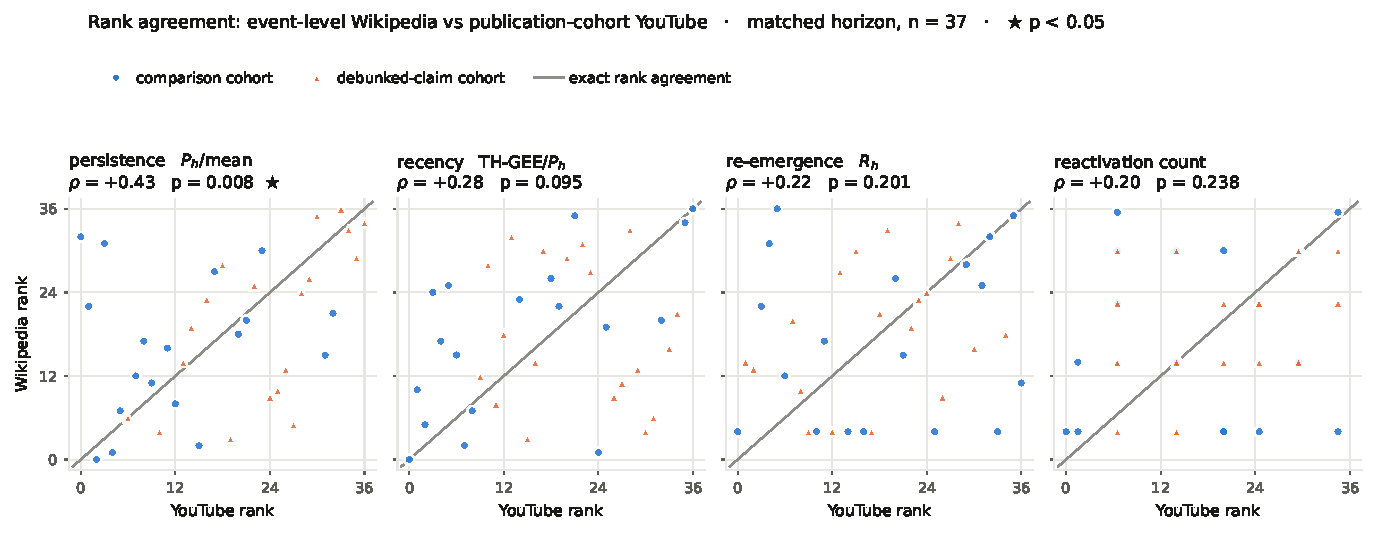
\includegraphics[width=\textwidth]{wikipedia_vs_youtube.pdf}
\caption{Rank-rank agreement for each scale-free indicator under the primary
specification. Red points are debunked-claim cohorts. The dashed line is exact
rank agreement.}
\label{fig:or1_rankrank}
\end{figure*}

\subsection{RQ6 replicates at event level}
\label{sec:or1_rq6}

Although topic-level ranks agree weakly, the main text's substantive conclusion
about debunked-claim cohorts is a group-level claim, and it replicates.

At weekly resolution all 19 debunked-claim cohorts register at least two
qualifying reactivations, with $R_h$ between $0.013$ and $0.062$, reproducing the
main text's Section 5.6 finding on event-level data. They do not occupy a
distinctive region of profile space: 84\% of them fall inside the comparison
cohorts' persistence range, 100\% inside its recency range, and 79\% inside its
$R_h$ range (Figure~\ref{fig:or1_space}). The heterogeneity-and-overlap
conclusion of the main text is thus not an artifact of publication-cohort
measurement.

On the quarterly grid the same claim is weaker --- 16 of 19 cohorts show at least
one reactivation, but not all reach two --- which reflects the resolution
mismatch discussed next rather than a substantive difference.

\begin{figure*}[htbp]
\centering
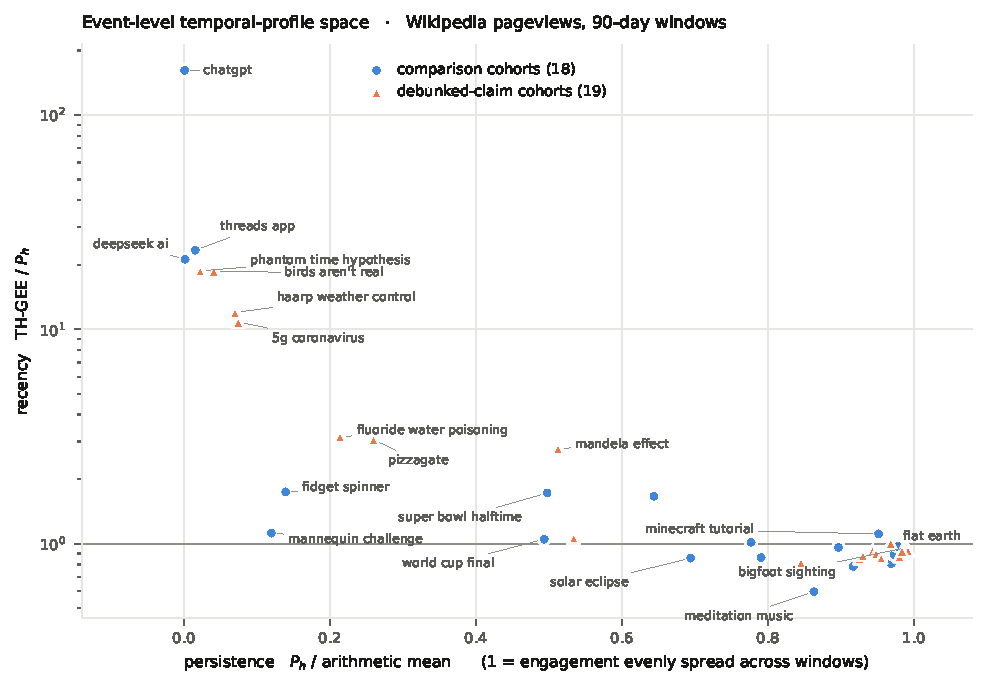
\includegraphics[width=0.86\textwidth]{wikipedia_profile_space.pdf}
\caption{Event-level temporal-profile space, the counterpart of main-text
Figure~2. The groups overlap as they do in the main text.}
\label{fig:or1_space}
\end{figure*}

\subsection{The activity threshold, not the construct, drives the re-emergence gap}
\label{sec:or1_qh}

The third panel of Figure~\ref{fig:or1_exemplars} is diagnostic. \emph{Solar
eclipse} carries two of the largest attention spikes in the entire dataset --- the
2017 and 2024 eclipses, each reaching roughly 24{,}000 views/day against a
baseline near 1{,}500 --- and yet records $R_h = 0.000$ with no qualifying
reactivations.

Under the framework's own definitions this is the correct answer. $R_h$ asks
whether activity \emph{returned after dormancy}, and a live Wikipedia article on
an evergreen subject is never dormant: its quiet quarters still sit above its own
25th percentile, so no dormant interval qualifies and the eclipses are bursts
rather than returns. The main text draws exactly this distinction when it notes
that continuously active content can score high on persistence and recency
without ever becoming dormant.

The consequence, however, is that on dense attention series the quartile rule
leaves $R_h$ structurally unable to respond to spike structure, because $q_h$ is
defined as a quantile of the topic's own distribution and a topic that is always
on has a high one. We therefore report an alternative \emph{elevation} rule,
$q_h = k \times \operatorname{median}(E_\tau)$, under which ``active'' means
elevated above the topic's own baseline rather than above its lower quartile.
This changes one parameter rule and nothing else in the framework.

The effect is large. Table~\ref{tab:or1_groups} shows that at weekly resolution
the elevation rule recovers the \emph{a priori} ordering of reactivation counts
--- re-emergent (23) $>$ acute (7) $>$ persistent (2) --- which the quartile rule
does not (10, 22, 21 respectively, with the persistent topics scoring
\emph{lowest} on a measure they should not lead). This is a construct-validity
result of the kind main-text Section 5.5 reports for YouTube, now on event-level
data.

We flag the status of this rule plainly: it was adopted after observing that the
quartile rule fails on dense data, so it is exploratory rather than confirmatory.
It is not, however, knife-edge in $k$. Over $k \in \{1.5, 2, 3, 4\}$ the burst
localisation lift below rises monotonically from $6.4\times$ to $17.6\times$
(all $p = 0.0001$), the rank correlation with change-point counts from $+0.51$ to
$+0.60$, and the \emph{a priori} group ordering holds at every value.

\subsection{OR2: agreement with the sequence-oriented baselines}
\label{sec:or1_or2}

Table~\ref{tab:or1_baselines} reports the comparison, and
Figure~\ref{fig:or1_bursts} draws all three objects on the same axis for four
topics.

Under the paper's quartile $q_h$ on the quarterly grid there is no agreement with
Kleinberg at all (lift $1.0\times$, $p = 0.51$) and only a weak one with PELT
($1.4\times$, $p = 0.079$). Moving to weekly windows raises both to about twice
chance ($1.96\times$, $p = 0.015$; $2.18\times$, $p = 0.0002$).

Under the elevation rule at weekly resolution the agreement becomes substantial.
Reactivation windows contain a Kleinberg burst onset $10.7\times$ more often than
a uniformly chosen window ($63/351$, $p = 0.0001$) and a PELT change point
$6.6\times$ more often ($68/351$, $p = 0.0001$). Across the 37 topics the
reactivation count correlates with the change-point count at $\rho = +0.56$
($p = 0.0003$) and with the burst count at $\rho = +0.27$.

Two limits of this agreement should be stated alongside it. First, recall is low:
reactivation windows contain only 20\% of detected burst onsets and 13\% of
change points, so $R_h$ sees a minority of what the event-level detectors find.
Second, $R_h$ correlates \emph{negatively} with total burst duration
($\rho = -0.32$), which is as it should be --- a topic that spends most of the
horizon in an elevated state has few returns to detect --- but it confirms that
$R_h$ and burst detection are not measuring the same quantity.

The answer to OR2 is therefore that the Re-Emergence Index is genuinely
concordant with methods built for event-level data, at six to eleven times
chance, provided the activity threshold is specified for the density of the data.
It remains a coarser and more selective instrument than either baseline, which is
consistent with the main text's positioning of TH-GEE as an interpretable summary
that complements rather than replaces sequence-oriented approaches.

\begin{figure*}[htbp]
\centering
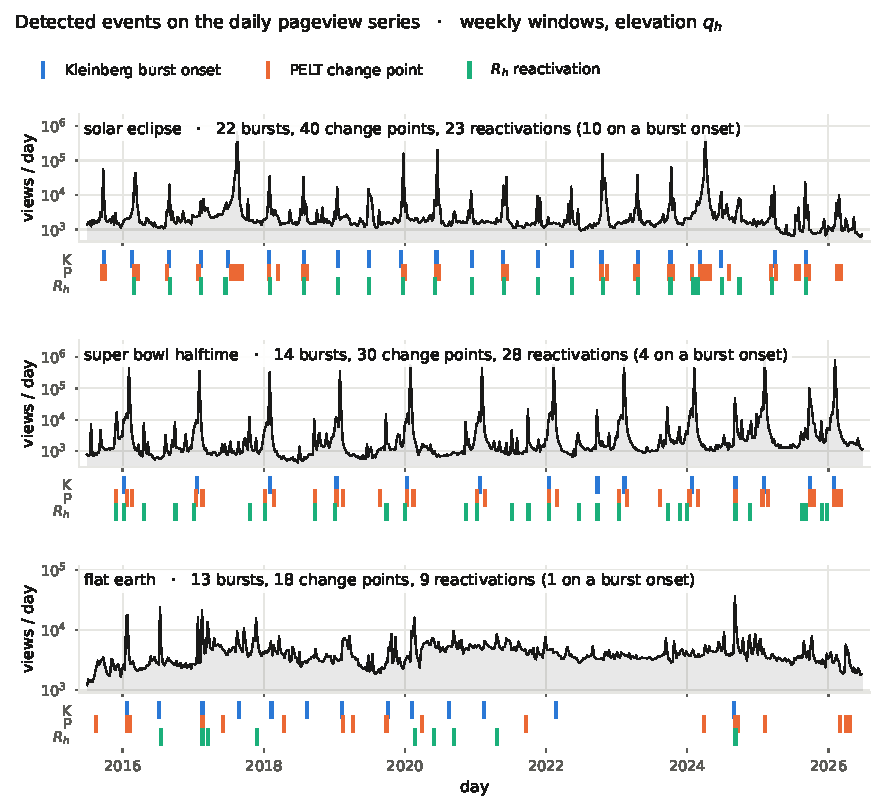
\includegraphics[width=\textwidth]{wikipedia_bursts.pdf}
\caption{Daily pageviews (log scale) with Kleinberg burst onsets, PELT change
points, and $R_h$ reactivation windows on a common axis, under the weekly
elevation specification. The annual periodicity of \emph{super bowl halftime} and
the eclipse spikes in \emph{solar eclipse} are picked up by all three.}
\label{fig:or1_bursts}
\end{figure*}

\subsection{Sensitivity checks}
\label{sec:or1_sensitivity}

\paragraph{Window length and span.}
All seven specifications appear in Table~\ref{tab:or1_agreement}. No conclusion
above rests on a single window length: the persistence result is reported
together with the own-span control that weakens it, and the re-emergence null
holds at every window length tested.

\paragraph{Mapping fidelity.}
Restricting to the 31 high-fidelity mappings never reverses a sign and generally
strengthens the correlations slightly (persistence $+0.43 \to +0.50$ on the
primary specification), which is what one expects if imperfect mapping adds noise
rather than bias.

\paragraph{Alternative articles.}
For the eight topics with a defensible alternative article the profiles are
recomputed on both. Four are essentially unaffected (persistence ratio moving by
$0.08$ or less), and four move materially, in every case for an interpretable
reason: the alternative is a broader article that adds off-topic traffic and
therefore looks flatter. The largest shift is \emph{fluoride water poisoning},
where \emph{Opposition to water fluoridation} ($P_h/\bar{E} = 0.21$) is replaced
by the general \emph{Water fluoridation} article ($0.90$), followed by
\emph{yoga for beginners} ($0.64 \to 0.94$), \emph{world cup final}
($0.49 \to 0.74$) and \emph{mandela effect} ($0.51 \to 0.74$). This is why the
narrower, topic-specific article is the primary mapping throughout and why the
high-fidelity subset is reported separately; no group-level conclusion changes
under either choice.

\input{or1_tables}

\section{Limitations}
\label{sec:or1_limits}

\paragraph{A pageview is not a YouTube engagement.}
The two platforms measure different acts. A pageview is a single retrieval by a
reader who has already decided to look something up; a YouTube like or comment is
a deliberate, costlier signal attached to a specific video. Agreement between the
two profiles is evidence that the \emph{temporal structure} of attention to a
topic is a property of the topic rather than of one platform's measurement
apparatus. It is not evidence that the two platforms' audiences behave alike, and
disagreement on any single topic can reflect a genuine difference in how that
topic is consumed on each platform.

\paragraph{Mapping is one-to-many and imperfect.}
A YouTube search term retrieves a cohort of videos; a Wikipedia article is one
document. Broad articles carry off-topic traffic (\emph{CERN} is mostly about
particle physics, \emph{Area 51} mostly about the airbase), and narrow search
terms have no exact article counterpart. This is why every mapping carries a
fidelity grade and every agreement statistic is reported both for all 37 topics
and for the high-fidelity subset.

\paragraph{The horizon floor is binding for the acute exemplars.}
As noted in Section~\ref{sec:or1_horizon}, per-article pageviews start
2015-07-01, so fads that peaked before that date are observed only in decline.

\paragraph{Wikipedia has its own visibility mechanics.}
Pageviews are shaped by search-engine ranking, the Wikipedia main page, mobile
app surfacing, and internal linking, exactly as YouTube engagement is shaped by
recommendation. Event-level timing removes the publication-cohort confound; it
does not remove platform mediation.

\paragraph{No causal claim.}
As in the main text, these are descriptive measurements of observable attention.
Nothing here establishes belief, persuasion, intent, coordination, or veracity.

\end{document}
